In the diagram below, $ABCD$ is a square. Point $E$ is the midpoint of $\overline{AD}$. Points $F$ and $G$ lie on $\overline{CE}$, and $H$ and $J$ lie on $\overline{AB}$ and $\overline{BC}$, respectively, so that $FGHJ$ is a square. Points $K$ and $L$ lie on $\overline{GH}$, and $M$ and $N$ lie on $\overline{AD}$ and $\overline{AB}$, respectively, so that $KLMN$ is a square. The area of $KLMN$ is 99. Find the area of $FGHJ$.
\begin{center}
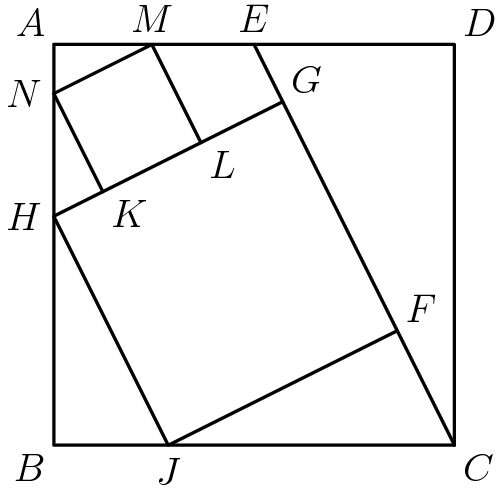
\includegraphics[width = 50.400000000000006mm]{img/fig0.png}
\end{center}